\documentclass[9pt,twocolumn,twoside]{../../styles/osajnl}
\usepackage{fancyvrb}
\usepackage{graphicx}
\usepackage{hyperref}
\usepackage{color}
\usepackage{listings}
\lstdefinestyle{BashInputStyle}{
  language=bash,
  basicstyle=\small\sffamily,
  numbers=left,
  numberstyle=\tiny,
  numbersep=3pt,
  frame=tb,
  columns=fullflexible,
  backgroundcolor=\color{yellow!20},
  linewidth=0.9\linewidth,
  xleftmargin=0.1\linewidth
}
% \graphicspath{ {images/} }
\journal{i524} 

\title{Remotely Deploying, Visualizing and Controlling a Robot Swarm with ROS}

\author[1]{Matthew Lawson}
\author[1,*]{Gregor von Laszewski}

\affil[1]{School of Informatics and Computing, Bloomington, IN 47408, U.S.A.}

\affil[*]{Corresponding authors: laszewski@gmail.com}

\dates{project-000, \today}

\ociscodes{Cloud, I524, ROS, Gazebo, Robot, Swarm}

% replace this with your url in github/gitlab
\doi{\url{https://github.com/cloudmesh/sp17-i524/tree/master/project/S17-IO-3010/report/report.pdf}}
% \doi{\url{https://github.com/cloudmesh/cloudmesh.ros/master/report/report.pdf}}

\begin{abstract}
Our project demonstrates the feasibility of harnessing remotely-located distributed computing environments, i.e., "clouds", to simulate large-scale robot swarms.  Our proof-of-concept program creates a two-robot swarm on a cluster of remotely-located computers.  It then pushes a visual simulation of the robots to the remote user.  Finally, it sends a single command to the robots in order to demonstrate the feasibility of networked communication with the robots.  The project utilizes two software packages from the Open Source Robotics Foundation (OSRF).  Namely, it uses the \textit{Robot Operating System} to define, create and control the virtual robots.  The OSRF's \textit{Gazebo} simulation software provides visualization of the simulation.  We use \textit{cloudmesh}, \textit{Ansible} and a *nix shell script to deploy the software to a distributed computing environment.
\newline
\end{abstract}

\setboolean{displaycopyright}{true}

\begin{document}

\maketitle

\section{Introduction}
Simulating a single robot's actions and responses to its environment prior to real-world deployment mitigates risk and improves results at a relatively low cost. Therefore, it seems reasonable to conclude that simulating the actions and responses of a group of robots, e.g., a swarm, will also improve results at a low cost.  However, deployment of an interconnected swarm of virtual robots on a remotely-located cluster of computers imposes additional requirements versus a locally-hosted single- or multi-robot deployment.  For instance, accessing and configuring multiple computers presents a time and resource challenge in contrast to a single-host setup.  In addition, network security measures, such as ssh keys and port access, impede ROS' intra-cluster communication capabilities.  In order to address the unique requirements of a networked, remotely-located swarm, we create a multi-platform system to automate the creation and deployment of the virtual swarm. 

\section{Virtual Robot Swarm Components}

\subsection{Robot Operating System (ROS)} % \cite{www-ros-about}}
% TBD; will include a discussion of a) how to obtain and install ROS and b) ROS graph concepts.  The latter topic will introduce ROS' core components, namely a node, publications, suscriptions, topics and services.  This section should probably cover ROS packages and ROS client libraries (primarily C++ and Python)

\begin{figure*}[htbp]
\centering
\fbox{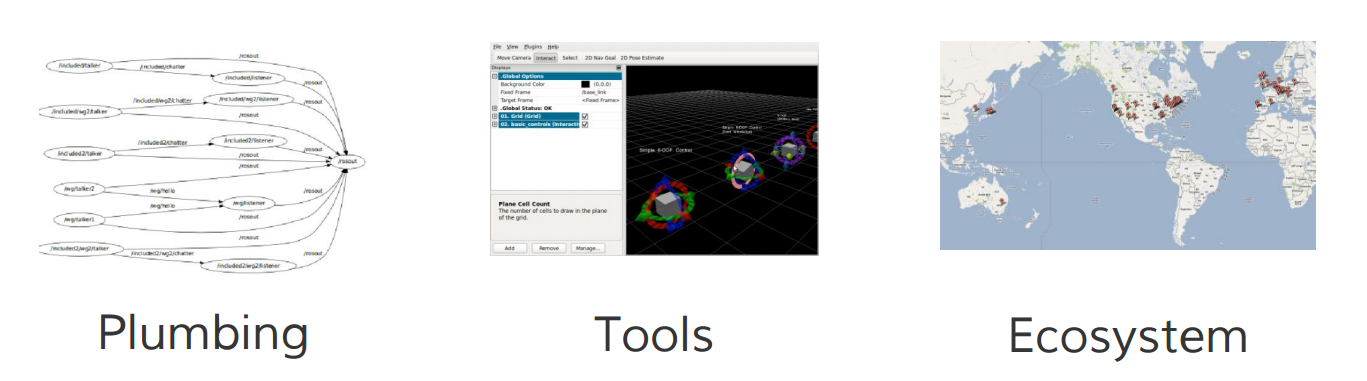
\includegraphics[width=\linewidth]{images/ros-is.png}}
\caption{A Conceptualization of What ROS, the \textit{R}obot \textit{O}perating \textit{S}ystem, Offers to Roboticists \cite{www-ros-ros-is}}
\label{fig:rosOverview}
\end{figure*}

\begin{figure}[htbp]
\centering
\fbox{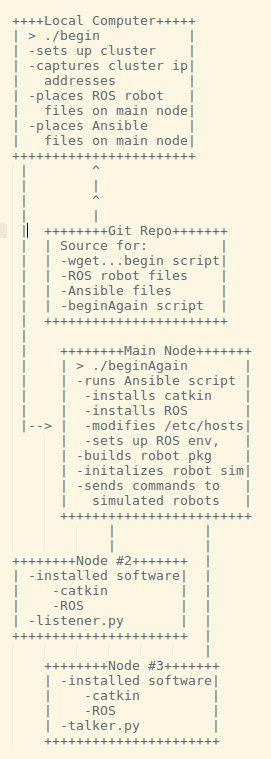
\includegraphics[width=\linewidth]{images/deployWorkFlowCol.jpeg}}
\caption{Deployment Workflow for the Virtual Robot Swarm Project}
\label{fig:deployWorkflow}
\end{figure}

The Open Source Robotics Foundation's middleware product \textit{Robot Operating System}, or ROS, provides a framework for writing operating systems for robots.  ROS offers "a collection of tools, libraries, and conventions [meant to] simplify the task of creating complex and robust robot behavior across a wide variety of robotic platforms" \cite{www-ros-about}. The Open Source Robotics Foundation, hereinafter OSRF or the Foundation, attempts to meet the aforementioned objective by implementing ROS as a modular system.  That is, ROS offers a core set of features, such as inter-process communication, that work with or without pre-existing, self-contained components for other tasks.

Figure 1 illustrates the ROS universe in three parts: a) the plumbing, ROS' communications infrastructure; b) the tools, such as ROS' visualization capabilities or its hardware drivers; and c) ROS' ecosystem, which represents ROS' core developers and maintainers, its contributors and its user base.

The modules or packages, which are analogous to packages in Linux repositories or libraries in other software distributions such as \textit{R}, provide solutions for numerous robot-related challenges.  General categories include a) drivers, such as sensor and actuator interfaces; b) platforms, for steering and image processing, etc.; c) algorithms, for task planning and obstacle avoidance; and, d) user interfaces, such as tele-operation and sensor data display. \cite{www-software-categories}

\subsection{Gazebo} % \cite{www-software-categories}}
% TBD; again, introducing core Gazebo concepts.  In this case, will include a) world files, b) model files and c) its client-server model.  It should also include non-obvious limitation examples, e.g., a gripper arm driven by a single screw instead of multiple screws.  In addition, it should allude to any limitations that affect our simulation.

The Foundation also supports \textit{Gazebo}, ROS' 3D virtual simulation software.  "Gazebo...simulate[s] populations of robots in complex indoor and outdoor environments. [It] offers physics simulation at a much higher degree of fidelity [than gaming engines], a suite of sensors, and interfaces for both users and programs \cite{www-gazebo-overview}."  Gazebo's usefulness center on three main features: a) physics engines compatibility; b) its graphics engine; and c) its sensor-data generators.  with respect to physics engine compatibility Gazebo interfaces well with \textit{Open Dynamics Engine} \cite{www-ode-homepage} (ODE), the default; b) \textit{Bullet} \cite{www-bullet-homepage}; \textit{SimBody} \cite{www-simbody-homepage}; and, \textit{DART} \cite{www-dart-homepage}. Roboticists also benefit from its 3D graphics engine, \textit{Object-oriented Graphics Rendering Engine} \cite{www-ogre-homepage} (OGRE), which provides a C++ class library to "[abstract away] the details of using the underlying [graphics] system libraries like Direct3D and OpenGL \cite{www-ogre-about}."  Finally, Gazebo can supply \textit{sensor} data to the virtual robot.  Virtual sensor support ranges from 2D cameras to Kinect-style sensors.  The system can also generate \textit{noisy} data to better simulate real-world results.

Gazebo exists as a stand-alone project, suitable for use by programs other than ROS.  However, it integrates tightly with ROS given its common ownership.  In fact, the version supplied with a ROS installation automatically establishes communications between Gazebo and ROS for the end-user \cite{www-gazebo-ros}.  

\subsection{Ansible}
% TBD; briefly describe Ansible - what it is, salient features, etc.

Red Hat, Inc's \cite{www-redhat} \textit{Ansible} software purports to simplify numerous information technology tasks.  It claims to do so by a) relying upon a human-readable script syntax, YAML; and b) by automating definable and repeatable IT tasks, such as configuration management and application deployment.  Ansible's developers adopted a theater metaphor to describe the program's core functions.  Thus, a computer's main duty within an IT infrastructure corresponds to the \textit{role} an actor or actress might play in a theatrical production.  Ansible calls the script a \textit{playbook}, while the lines and directions within the script are referred to as \textit{tasks}.  Other aspects diverge from the metaphor, such as group vars and the config file (ansible.cfg).  However, the \textit{inventory} file hews to the metaphor - it represents the cast billing, the delineation of who plays what role.  When used with an Ansible playbook, the inventory file specifies which servers belong to which logical group(s), i.e., which role(s). 

As a result the software's applicability extends well beyond simplistic tasks even though Ansible's designers strive for simplification.  In fact, an Ansible user can exercise fine-grained control over nearly every aspect of his or her IT infrastructure with a well-designed playbook.  

Ansible also attempts to ease the burden of the IT administrator by eschewing SSL signing servers, daemons or client software.  It simply pushes small programs to the target computers through an SSH connection to execute the desired tasks.  When the task completes, Ansible removes the programs. 

\subsection{cloudmesh client toolkit}
The \textit{cloudmesh client toolkit} (cm) attempts to abstract away the complexities of establishing and utilizing different remotely-accessed computers and computer clusters \cite{www-cm}.  Users can create, access and destroy a virtual machine or cluster of machines by issuing a single line of commands from a terminal emulator.  cm supports access to clouds based on various back end-software stacks, including SLURM, SSH, Openstack and Heat.  It provides an API, a command line client and a shell client.

\subsection{Testing Environment}
The Chameleon project's cluster of 650+ multi-core computer nodes, a joint venture between the University of Chicago and the Texas Advanced Computing Center, provides the infrastructre for the project.  It is colloquially referred to as Chameleon Cloud or CC.  A 100Gbps connection runs between the two centers. Project development primarily occurred on three-node clusters created as needed using Chameleon Cloud's \textit{m1.medium flavor} of Ubuntu 16.04.  The m1.medium flavor's resources consist of two virtual CPUs, 40GB of hard drive space and 4GB of RAM.  

\subsection{Robots and Worlds}
A ROS robot may be extremely simple, such as the pre-built talker and listener robots supplied in the ROS distribution, or as complex as the roboticist desires.  If users desire to visualize the robot, s/he must define his / her ROS robot in \textit{\textbf{U}niversal \textbf{R}obot \textbf{D}escription \textbf{F}ormat}.  A ROS robot's specifications reside in a series of files with \textit{xacro} extensions, referred to as URDF files.  These files, which borrow XML's syntax structure, can include specifications for the basic shapes of the robot and its appendages (if applicable), e.g., rectangular box, cylinder, etc. with attached wheels, various kinds of joints, such as ones that rotate around an axis or extend along an axis, types and numbers of sensors, number of joints in an appendage, colors of the robot(s), etc., etc.  In addition, any file in the robot description stack may reference an external file to complete the description of the robot.  This capability allows the user to re-use code by incorporating previously-completed robot features into a new robot.  Finally, simulations include a world file to provide the setting, or environment, in which the robot simulation occurs.  As with the URDF files, the world file can be simple, like the \textit{empty\_world} file included in the ROS distribution or extremely complex.  

Finally, a simulation package will include one or more \textit{launch} files.  These files coordinate the disparate aspects of the entire simulation package in a manner similar to that of Ansible's playbook file.  According to the OSRF, best practices for robot simulation dictate that the main launch file consist of little more than calls to other launch files in the package \cite{www-ros-launch}.  Continuing with the playbook analogy, the launch files called from the main launch file would correspond to the roles defined in Ansible.  This functionality significantly increases ROS' usability since managing even relatively straightforward robots, simulated or real, can prove unwieldy. For instance, this project, a proof-of-concept project, utilizes a .world file, four URDF files and four launch files in addition to the pre-compiled talker and listener robots.  

This project uses two straightforward differential drive robots sourced from an online tutorial entitled \textit{Simulating Robot Models in ROS (part 1)} \cite{www-mybot-moore}

\section{Virtual Robot Swarm Project Implementation}
\subsection{VR Swarm task}
% TBD; discuss the task to be accomplished by the swarm, as well as how the information collected during task completion will be communicated back to the master node for collation and reporting.

Although the swarm accomplishes the seemingly-trivial task of driving in circles, the real accomplishment rests in proving the feasibility of automating the deployment of multiple controllable virtual robots on a remote cluster of computers and then visualizing them on a local computer.

\subsection{Deployment}
% TBD; document the Ansible steps needed to successfully deploy ROS and Gazebo on multiple computers;  will include references for obtaining major components, including adding new repositories if needed.
Achieving the aforementioned task requires coordinating a modestly-complex mix of shell commands, cloudmesh commands, Ansible commands and ROS / Gazebo commands. A shell script provides the automation for the shell, cloudmesh and ROS commands, while Ansible's \textit{playbook} functionality handles the Ansible-focused portion.  Only the initial step, retrieving and sourcing the shell script that begins the deployment process, requires user intervention.  However, if the user wants to listen to the talker robot (\textit{talker.py and listener.py}), s/he needs to follow the steps described in the README file.

\begin{figure}[htbp]
\centering
\fbox{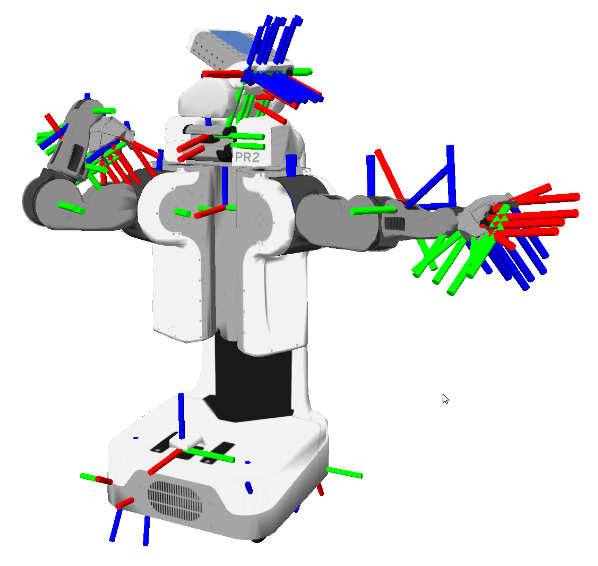
\includegraphics[width=\linewidth]{images/robotgeometry.png}}
\caption{Example of a Complex Simulated Robot}
\label{fig:complexRobot}
\end{figure}

\begin{figure}[htbp]
\centering
\fbox{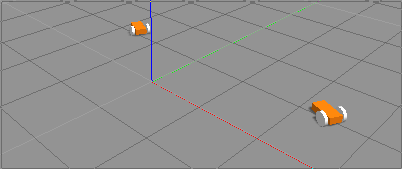
\includegraphics[width=\linewidth]{images/rosProjRobots.png}}
\caption{An Example of Two Simpler Robots}
\label{fig:simplerRobots}
\end{figure}

\paragraph{\textit{wget...begin} - Retrieve the Initalization Bash Script}
Deployment begins when the user retrieves the initalization file, named \textit{begin}, from the project's Github repository.  The user then starts the execution sequence by sourcing the file with the command \newline
{\color{green} \lstinline[style=BashInputStyle]!> ./begin! } \newline
from the directory where the \textit{begin} bash script resides.  

\paragraph{\textit{begin} bash script}
The bash script calls three cloudmesh\_client commands, {\color{green} \lstinline[style=BashInputStyle]!> cm cluster define -n rosA1 -c 3! }, {\color{green} \lstinline[style=BashInputStyle]!> cm cluster allocate! } and {\color{green} \lstinline[style=BashInputStyle]!> cm cluster cross_ssh! } in order to create and prepare the three-node cluster named \textit{rosA1}.  The script then uses two additional Cloudmesh commands, {\color{green} \lstinline[style=BashInputStyle]!> cm cluster nodes! } and {\color{green} \lstinline[style=BashInputStyle]!> cm vm ip show! } to capture the public and private ip addresses of the cluster as well as the host names.  

The ip addresses and names are written to separate files for distinct purposes.  The host names and private ip addresses are used to create a file to append to each cluster node's \textit{known\_hosts} file.  The private ip addresses also end up in a different file that serves as the basis for a custom Ansible inventory file.  

The private ip addresses, termed static ips by Chameleon, must be used because ROS nodes communicate by binding to any available port.  That is, ROS does not specify the port beforehand, and it does not consider whether or not the firewall blocks the port for security purposes.  As a result, intra-cluster communication requires access to every port, i.e., the firewall cannot close any port on any computer running ROS when that computer needs to communicate with another computer in the cluster.  Obviously, this presents a major security concern, especially on shared resources. Refer to the \textit{Common Pitfalls} section below for the workaround used with this project.

As its penultimate step, the \textit{begin} script places all the necessary files for the demonstration on the correct cluster nodes.  The ROS robot files and the Ansible files go onto the main node, while the script places a copy of the known\_hosts addendum onto each cluster node.  In addition, the script uses the \textit{wget} command to copy the bash script for the next step in the process onto the main node.

The final lines of the file initiate the next step in the process and perform a few administrative duties.

\paragraph{\textit{beginAgain} bash script}
This script handles the software installation and initialization of the robots.  It first establishes the veracity of the main node and the other nodes by connecting to each one in turn via ssh connection.  If these steps do not occur before Ansible runs, the software installations never occur because Ansible hangs mid-process.  Ansible installs all the necessary software on each cluster node.  It installs Linux's \textit{tree} package because the author prefers to use it to view directory structures; the ROS package; the rosbash package; the rosinstall package; and, the catkin\_tools package. Ansible also creates a new known\_hosts file for each computer node.

Upon completing the installation, the file's instructions initialize the robot workspace.  The \textit{catkin\_tools} package accomplishes this on behalf of ROS.  catkin\_tools represents an evolution of ROS' built-in \textit{catkin} family of commands.  Initializing the robot workspace essentially involves the addition of numerous hidden helper files, which assist in building the robot package.  Creating the robot package, referred to as \textit{building} the package, involves a series of automated \textit{CMake} commands.  

With the robot package built, the script copies another script from github.  This small script starts ROS' \textit{talker} robot, a simple robot included as part of ROS' tutorial packages.  It relies upon Linux's \textit{byobu} program to set up usable working environment if the user chooses to start the listener robot on the third cluster node.

Finally, execution of the last few lines of the script occurs.  These lines start ROS, start the two robots, create a simulated world for the robots and then issue a command for the robots to drive in circles.  Gazebo's simulation of the robots and their world come back through the ssh connection to the end user so s/he can see the simulation in real time. 

\paragraph{\textit{talkListen} bash script}
The \textit{talkListen} script sets up a multiplexed terminal environment on the second node and starts ROS' talker robot, which ROS' maintainers include as a pre-built package with the distribution.  It relies upon Linux's \textit{byobu} terminal multiplexing program.  Using a series of {\color{green} \lstinline[style=BashInputStyle]!> byobu-tmux ...! } commands, it creates a terminal screen with three panels.  ROS's rosmaster program starts in panel 1, while the talker program/robot/node starts in Panel 2.  The final panel, panel 0, connects to the third node in the cluster in anticipation of the user starting the listener program (also included in the ROS distribution).

\begin{figure*}[htbp]
\centering
\fbox{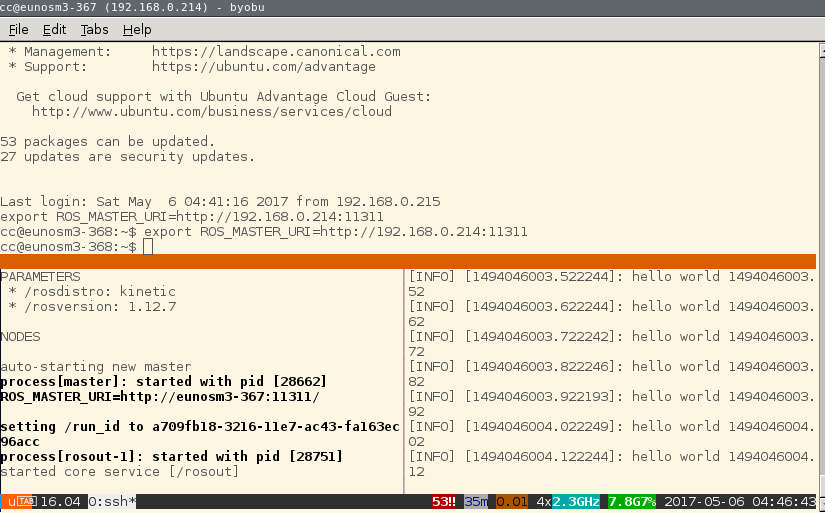
\includegraphics[width=0.75\textwidth]{images/byobu.png}}
\caption{The Multiplexed Talk-Listen Terminal}
\label{fig:byobu}
\end{figure*}

\subsection{Common Pitfalls}
% TBD; discuss any obstacles encountered with deployment due to dependency problems, connecting ROS and Gazebo, etc.
\paragraph{Intra-Node Communication}
In order to maintain security and enable intra-cluster communication, two of the three computer nodes must have their public ip addresses removed, i.e., disassociated, using Chameleon's browser-based graphical user interface (GUI), Horizon.  Then, and only then, the ports can be opened by applying the \textit{ros} security group to the two nodes in question (the private nodes).  Since the third node, the main node, still has a public-facing ip address, the other two nodes can be accessed via an ssh connection (\textit{ssh'ing}) to the main node and then ssh'ing to one of the private nodes.

\paragraph{Deployment Problems}
Even if a script or a user completes each step correctly to set up a controllable virtual swarm on remotely-located resources, problems still occur that cause deployment failures.  Usually, the issues can be resolved with manual intervention, so the deployment can be completed.  

\subparagraph{Adding the ROS Repository Key}
The deployment often goes awry during the Ansible script to retrieve the repository key for the ROS repo.  When the key retrieval failed, the ROS software installation would also fail.  Obviously, if the main node lacks ROS, the simulation will not launch either.  As a workaround, the script adds the repository to each machine with the \textit{deb [trusted=yes] ...} syntax.  Using this method obviates the need for the repo key.  Although it works, applying it to repos in general creates unnecessary risks.  Therefore, it should be used sparingly.  

\subparagraph{Starting the Robot Simulation}
Receiving an error while starting the simulation occurred much more frequently during the development process than the key repo problem.  ROS prints error messages in red to the console, so they stand out.  The most common error: {\color{red} \lstinline[style=BashInputStyle]![gazebo_gui-3] process has died! }.  Sometimes, an almost identical error occurs, {\color{red} \lstinline[style=BashInputStyle]![gazebo-2] process has died! }, while other times the launch program cannot find parts of the robot model.  The latter error consists of one or both of the following: {\color{red} \lstinline[style=BashInputStyle]!Error [parser.cc:581]! }{\lstinline[style=BashInputStyle]!Unable to find uri[model://ground_plane! } and / or {\color{red} \lstinline[style=BashInputStyle]!Error [parser.cc:581]! }{\lstinline[style=BashInputStyle]!Unable to find uri[model://sun! }.  Unlike the previously-described error, this one requires manual intervention.  The user needs to enter the following commands at the terminal prompt: a) {\color{green} \lstinline[style=BashInputStyle]!> killall roscore! }, b) {\color{green} \lstinline[style=BashInputStyle]!> killall rosmaster! }; c) {\color{green} \lstinline[style=BashInputStyle]!> killall gzclient! }; d) {\color{green} \lstinline[style=BashInputStyle]!> killall gzserver! }; e) {\color{green} \lstinline[style=BashInputStyle]!> source ~/.bashrc! }; and, {\color{green} \lstinline[style=BashInputStyle]!> ./beginAgain! }. Somewhat maddeningly, this process often needs to be completed twice before the simulation will start successfully.  If the simulation still will not start, refer to the instructions in the \textit{Initializing the Swarm} section.

\subsection{Initializing the Swarm Manually}
% TBD; starting ROS and Gazebo to create the virtual environment; testing swarm interconnectivity; designating master node, etc.
If needed the user can manually start the simulation with the commands listed below.  You will need three terminals for the three commands, so ssh into the main node three times from three separate consoles or use \textit{byobu} to split the terminal into three panes.  The command {\color{green} \lstinline[style=BashInputStyle]!> roslaunch mybot_gazebo mybot_world.launch! } starts the simulation.  Entering {\color{green} \lstinline[style=BashInputStyle]!rostopic pub /robot1/cmd_vel geometry_msgs/Twist '{linear: { !} {\color{green} \lstinline[style=BashInputStyle]!x: 0.2, y: 0.0, z: 0.0}, angular: {x: 0.0, y: 0.0, z: 0.1}}'! } \newline in a free terminal will command the first robot to begin turning in a circle.  Likewise, {\color{green} \lstinline[style=BashInputStyle]!rostopic pub /robot1/cmd_vel geometry_msgs/Twist '{linear: { !} {\color{green} \lstinline[style=BashInputStyle]!x: 0.2, y: 0.0, z: 0.0}, angular: {x: 0.0, y: 0.0, z: 0.1}}'! } \newline moves the second robot. Alternatively, one can delete the cluster and run the deployment script again.


\section{VR Swarm Project Conclusions}
TBD; present the data collected in some visualization format; discuss why this project advances robotics forward by utilizing distributed computing;

\section{Supplemental Material}

% Bibliography

\bibliography{references}
 
\section*{Author Biographies}
\begingroup
\setlength\intextsep{0pt}
\begin{minipage}[t][3.2cm][t]{1.0\columnwidth} % Adjust height [3.2cm] as required for separation of bio photos.
  \noindent
  {\bfseries Matthew Lawson} received his BSBA, Finance in 1999 from
  the University of Tennessee, Knoxville. His research interests include
  data analysis, visualization and behavioral finance.
\end{minipage}
\endgroup

\appendix
\begin{description}

\item[Matthew Lawson.] Designed the project in collaboration w/ Gregor von Laszewski, researched the material and implemented the project.  Slept far too little.

\item[Gregor von Laszewski.] Provided invaluable insights at key points during the process.

\end{description}

\end{document}
